\chapter{Results and analysis}\label{chapter:res-analysis}

\section{SPM and distgen}\label{section:spmydistgen}
This section will discussed the different scenarios that will be used for the testing of distgen as observed process. For an overview of Disgen, please refer to section \ref{section:distgen}.
\subsection{SPM and distgen with two threads}\label{subsection:spmydistgen-2t}

\subsubsection{Scenarios under consideration}\label{subsection:spmydistgen-2t-scens}

\begin{figure}
	\centering
		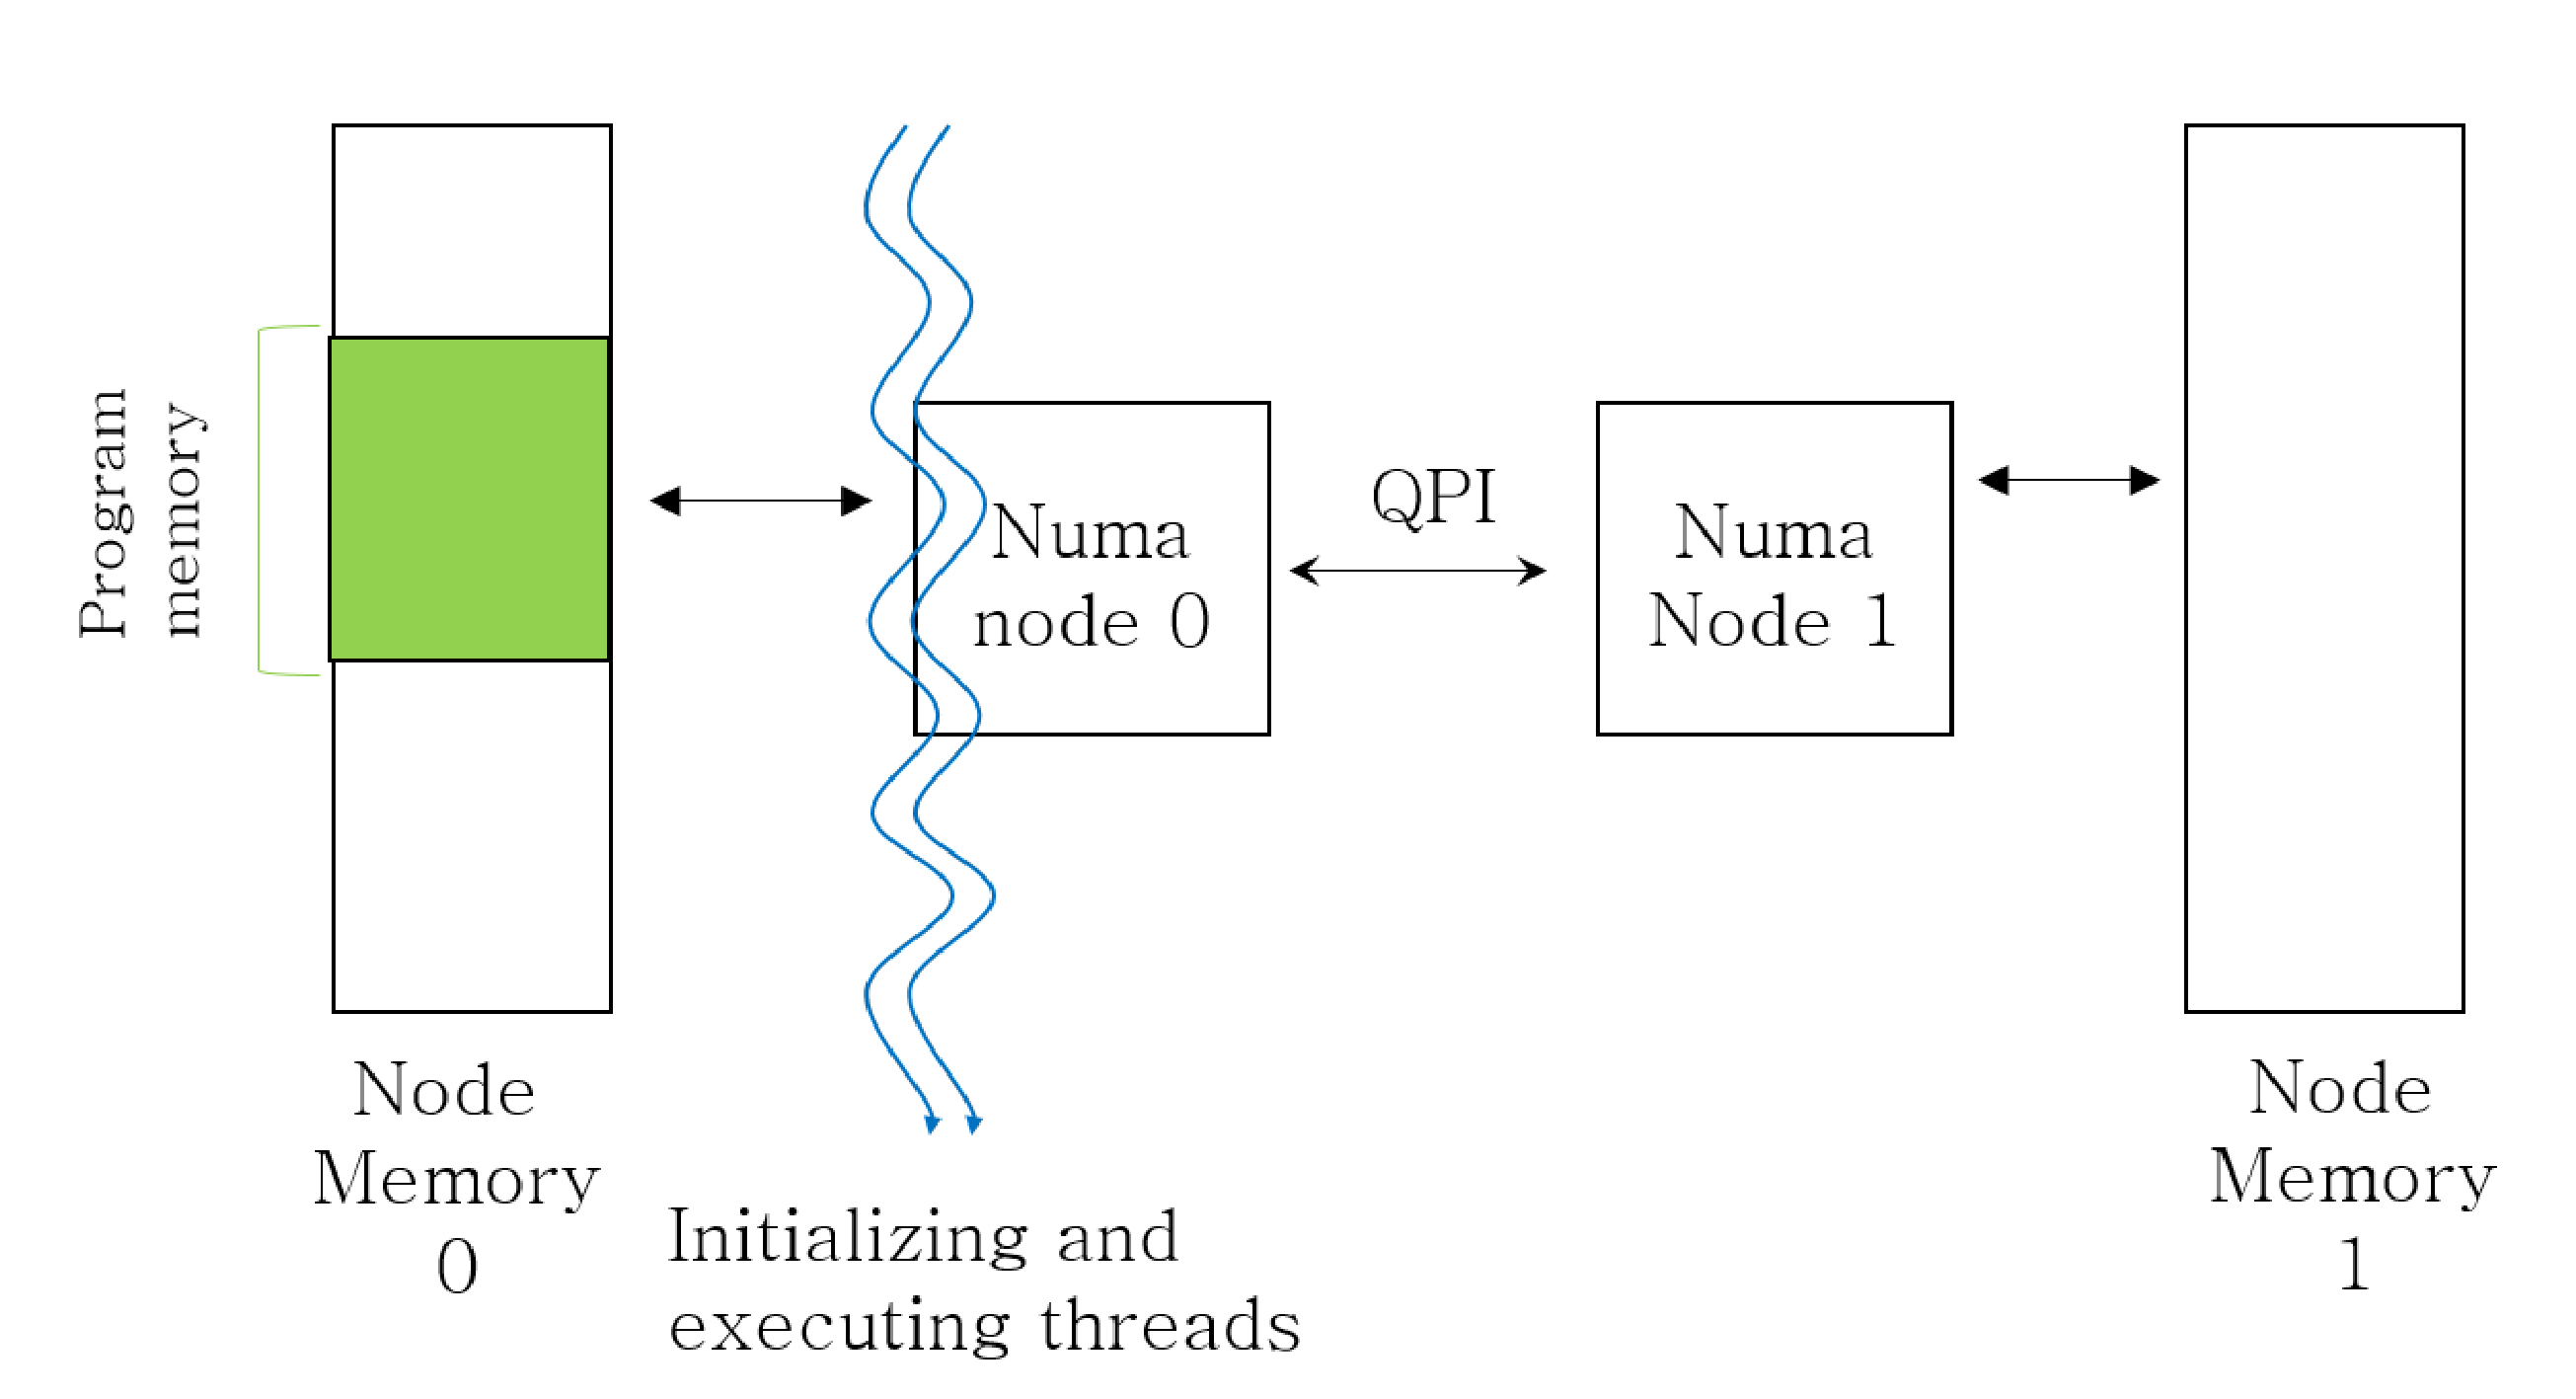
\includegraphics[width=.8\textwidth]{figures/distgentt-local.eps}
		\caption[Depiction of the working of the distgen vanilla local scenario with two threads]{Depiction of the distgen vanilla local with two running threads. Both threads are in the same NUMA node, therefore only local accesses will be performed.}
		\label{fig:dgentt-local}
\end{figure}

\begin{figure}
	\centering
		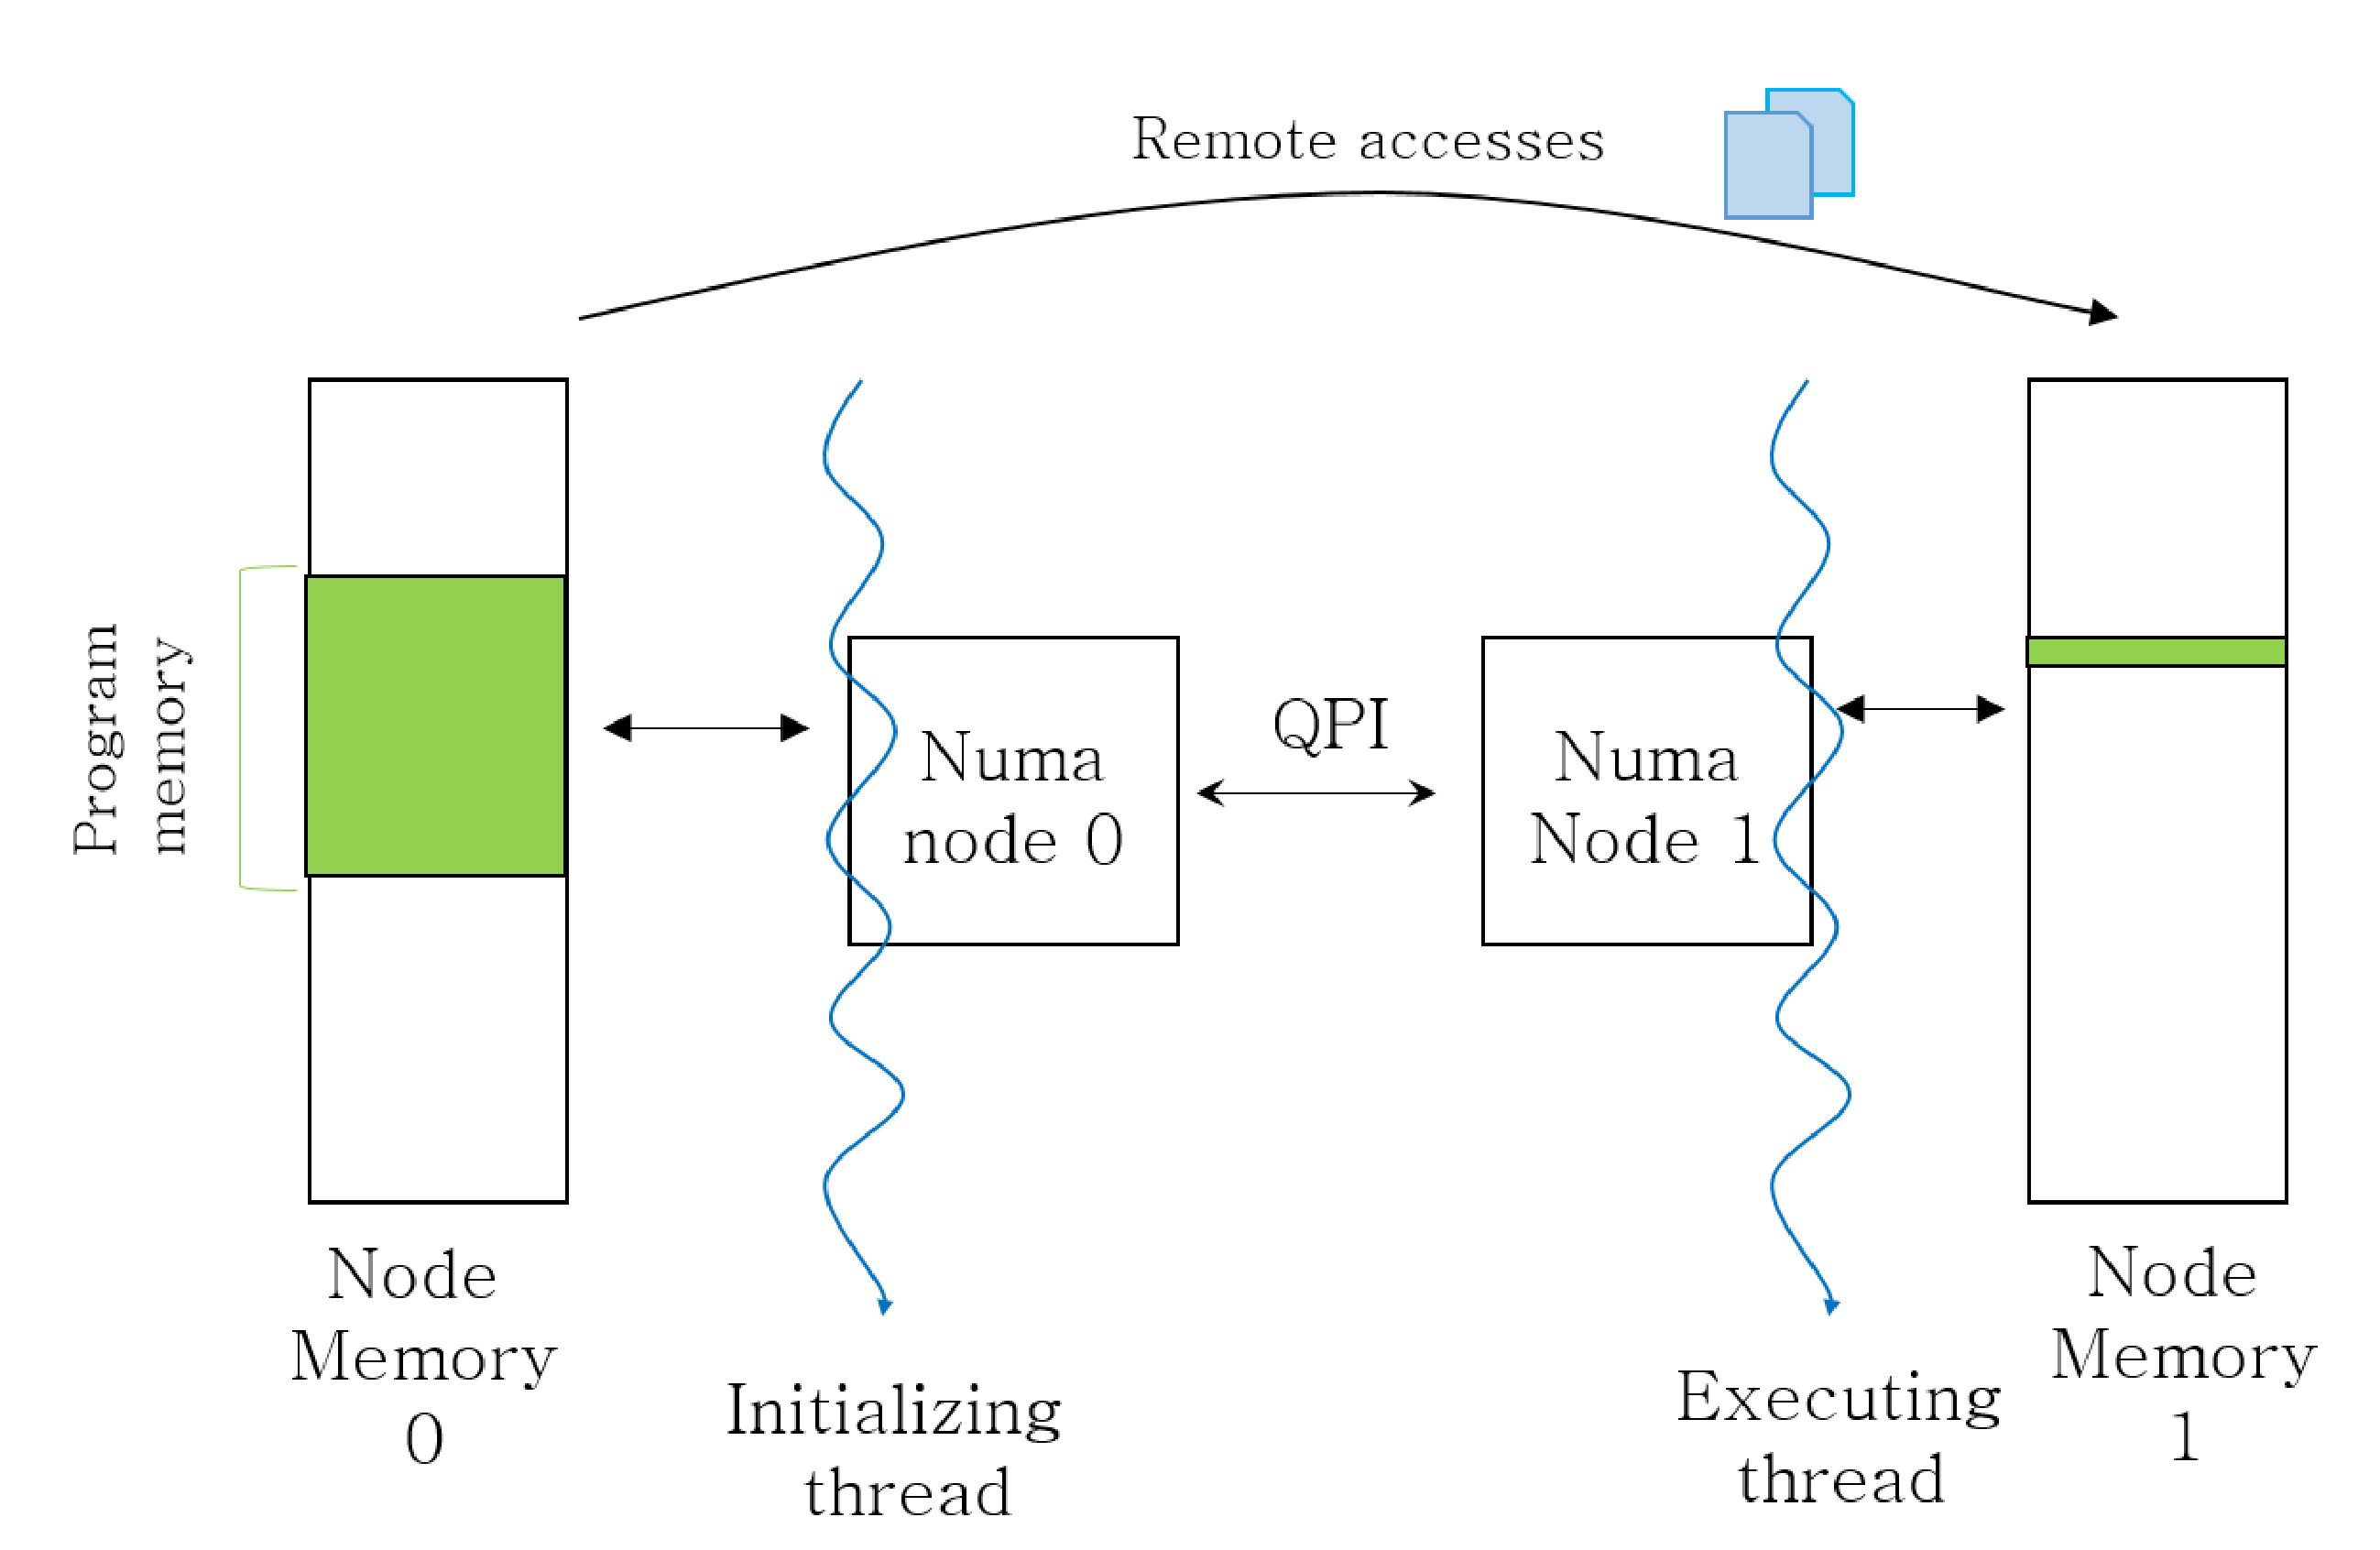
\includegraphics[width=.8\textwidth]{figures/distgentt-remote.eps}
		\caption[Depiction of the working of the distgen vanilla remote scenario with two threads]{Depiction of the distgen vanilla remote with two running threads. Each thread is pinned to a different NUMA node, which causes a lot of remote accesses to be done by the running thread.}
		\label{fig:dgentt-remote}
\end{figure}

\begin{itemize}
	\item The \textbf{vanilla local scenario} is the code in its original form, two threads are run in the same NUMA node.
	\item The \textbf{vanilla remote scenario}: Each thread runs on a separate NUMA node. The first thread initializes the memory space and the second thread accesses it. 
	\item The \textbf{SPM scenario} is the same as the vanilla remote scenario but this time the program execution will be overseen by the SPM tool and the pages observed to be accessed more from a remote node are moved to the node that originates the greater number of memory accesses.
	\item The \textbf{moveall} scenario is a distgen modification based on vanilla remote that after a determinate time of execution will move all the memory pages from a remote node to a local node.
\end{itemize}

Every one of this scenarios has a specific significance for the measurement of the performance: The vanilla local scenario shows the maximum speed possible for the given algorithm, Vanilla remote will show how much performance deteriorates when the algorithm is forced to perform many remote accesses in order to fetch the required data, moveall is a reference scenario that tells how much it is possible to fix the performance degradation by taking the pages placed in a remote node and bringing them close to the executing node and SPM also tries to fix the slowdown caused by the remote placement of the pages, but since the SPM does not know about the internal implementation of the supervised process, it will only move the pages that the PMU reports as remote accesses. The closer SPM's results are to the moveall scenario, the best performing the SPM tool is. Figures \ref{fig:dgentt-local} and \ref{fig:dgentt-remote} present depictions of both local and remote vanilla scenarios.

In order to be able to be able to place the pages remotely a modification has to be made to the original distgen code where the initialization is done by the master thread and the access is done only by the other thread, which is not the master. To determine whether the two threads are placed in a local node the environment variable \textit{GOMP\_CPU\_AFFINITY} is manipulated in order to determine the core in which the running threads will be placed. The availability of this modified two threads version is described in code listing 5 in Appendix \ref{app:coderes}.

